\documentclass[dvipdfmx]{article}
\setlength{\oddsidemargin}{-1.3truecm}
\setlength{\evensidemargin}{-1.3truecm}
\setlength{\textwidth}{18.5truecm}
\setlength{\headsep}{1truecm}
\setlength{\topmargin}{-2truecm}
\setlength{\textheight}{25truecm}
\usepackage{graphicx}
\DeclareGraphicsExtensions{.pdf}
\DeclareGraphicsExtensions{.eps}
\graphicspath{{out/}{out/tex/}{out/pdf/}{out/eps/}{out/tex/gpl/}{out/tex/svg/}{out/pdf/dot/}{out/pdf/gpl/}{out/pdf/img/}{out/pdf/odg/}{out/pdf/svg/}{out/eps/dot/}{out/eps/gpl/}{out/eps/img/}{out/eps/odg/}{out/eps/svg/}}
\usepackage{listings,jlisting}
\usepackage{fancybox}
\usepackage{hyperref}
\usepackage{color}

\newcommand{\bvec}[1]{\mbox{\boldmath $#1$}}

\lstset{language = python,
numbers = left,
numberstyle = {\tiny \emph},
numbersep = 10pt,
breaklines = true,
breakindent = 40pt,
frame = tlRB,
frameround = ffft,
framesep = 3pt,
rulesep = 1pt,
rulecolor = {\color{blue}},
rulesepcolor = {\color{blue}},
flexiblecolumns = true,
keepspaces = true,
basicstyle = \ttfamily\scriptsize,
identifierstyle = ,
commentstyle = ,
stringstyle = ,
showstringspaces = false,
tabsize = 4,
escapechar=\@,
}


\title{水素原子のシュレディンガー方程式を最も単純なやり方で解く}
\author{田浦}
\date{}

\begin{document}
\maketitle

\section{}
水素原子中の電子の波動関数$\phi(\bvec{x})$が満たす,
時間に依存しない方程式は,
\begin{equation}
\left(- \frac{\hbar^2}{2m} \nabla^2 + V(\bvec{x})\right) \phi(\bvec{x}) 
= E \phi(\bvec{x})
\end{equation}
ここで, 
\begin{equation}
  V(\bvec{x}) = - \frac{e^2}{4\pi \epsilon_0 |\bvec{x}|}
\end{equation}
なので結局, 
\begin{equation}
\left(- \frac{\hbar^2}{2m} 
\left(\frac{\partial^2}{\partial x^2} + \frac{\partial^2}{\partial y^2} + \frac{\partial^2}{\partial z^2} \right)
- \frac{e^2}{4\pi \epsilon_0 \sqrt{x^2 + y^2 + z^2}}\right)
\phi(x, y, z) = E \phi(x, y, z)
\label{eq:shrodinger}
\end{equation}
が解くべき方程式. 

\section{離散化}
解を求める空間を
\begin{equation}
[-a,a]^3 \equiv \{ (x,y,z) \;|\; -a \leq x, y, z \leq a \}
\end{equation}
とし, 一辺を$(n+1)$等分して離散化する
($x_{-1} = -a, x_{i+1} = x_i + 2a/(n+1), x_n = a$).
\begin{equation}
\phi_{i,j,k} \equiv \phi(x_i, y_j, z_k)
\end{equation}
と定義し, 式($\ref{eq:shrodinger}$)を離散化する. 例えば
\begin{equation}
\frac{\partial^2}{\partial x^2} \phi(x, y, z)
\approx
\frac{\phi(x + d, y, z) - 2\phi(x, y, z) + \phi(x - d, y, z)}{\Delta x^2}
\end{equation}
したがって, 
\begin{equation}
- \frac{\hbar^2}{2m \Delta x^2} 
\left(
  \phi_{i+1,j,k} + \phi_{i-1,j,k} 
+ \phi_{i,j+1,k} + \phi_{i,j-1,k} 
+ \phi_{i,j,k+1} + \phi_{i,j,k-1} 
- 6 \phi_{i,j,k}
\right)
- \frac{e^2}{4\pi \epsilon_0 \sqrt{x_i^2 + y_j^2 + z_k^2}}
\phi_{i,j,k}
= E \phi_{i,j,k}
\end{equation}
ただし$\Delta x = 2a/(n+1)$.

ただしい境界条件は無限遠で$\phi = 0$というものだが,考えている領域の
境界で0とする.

\section{Python化}
$\phi_{i,j,k}$を辞書順に並べたベクトルを$\phi$とする.

\[ \phi = {}^t(\phi_{0,0,0}\; \phi_{0,0,1}\; \cdots) \]

その約束のもと,左辺を
\[ H \phi \]
と書いた時, $H$に相当する行列を作ることだけが仕事で,
あとは固有値を求めるscipyの関数に放り込めば良い.

まず
\[
  \phi_{i+1,j,k} + \phi_{i-1,j,k} 
+ \phi_{i,j+1,k} + \phi_{i,j-1,k} 
+ \phi_{i,j,k+1} + \phi_{i,j,k-1} 
- 6 \phi_{i,j,k}
\]
を$L \phi$と書いた時の$L$は,
対角成分に $-6$, あとは非対角各成分に1を持つような
帯が6つ並ぶだけの行列で,scipyでは, 
diagsを用いて簡単に書ける.

\begin{lstlisting}
L = scipy.sparse.diags([-6.0,  1.0,  1.0,   1.0,  1.0,  1.0,  1.0 ], 
                       [   0,     1,   -1,    n,   -n,  n*n, -n*n ], 
                       shape=(n**3, n**3))
\end{lstlisting}

次に,
\[ 
\frac{1}{\sqrt{x_i^2 + y_j^2 + z_k^2}} \phi_{i,j,k}
\]
を$D \phi$と書いたときの$D$に相当する行列は,単なる対角行列で,
$\phi_{i,j,k}$に対する添字が
$1/\sqrt{x_i^2 + y_j^2 + z_k^2}$であるというもの.
$\phi_{i,j,k}$は$n^2 i + n j + k$番目の成分だからそれを用いて
その行列を作ることもできるが,もっと簡単なのはまず3次元配列として
作ってから1次元にreshapeするというやり方.

\begin{lstlisting}
l = np.linspace(-a, a, n+2)[1:-1]  # [-a,a]を(n+1)等分した内点n個
x,y,z = np.meshgrid(l, l, l)       # x,y,z それぞれが n x n x n 配列
V = 1.0 / np.sqrt(x*x+y*y+z*z)     # V も n x n x n (universal関数)
D = scipy.sparse.diags([ V.flatten() ], [ 0 ]) # flattenで1次元配列にする
\end{lstlisting}

上記のようにして$L$, $D$を得たら,
\[ H = -\frac{\hbar^2}{2 m \Delta x^2} L 
       - \frac{e^2}{4.0 \pi \epsilon_0} D 
\]
とすればよい.

ただし行列を目視で確認するときに絶対値の小さい値ばかりだと見難いので,
$L$の係数が1になるようにスケールさせておく.
\[ H' = -L 
       - \frac{m \Delta x^2 e^2}{2 \pi \epsilon_0 \hbar^2} D \]
付録のコードで計算しているのはこの$H'$である.

\section{固有値ソルバ}
{\tt scipy.sparse.linalg}に,
{\tt eigs} (一般の行列用), 
{\tt eigsh} (対称(半?)正定値行列用)の2種類がある.
対称は間違いないのだが,正定値かどうか確信のないまま
結果オーライで後者を使っている.

多数の固有値固有ベクトルのうち,どれを返すか({\tt which}),
いくつ返すか({\tt k})というオプションがあり,{\tt which}が重要.
algebraically smallest (つまり絶対値ではなく普通に符号を含めて
小さいものを選ぶ){\tt which='SA'}を用いる.{\tt k}は表示したいだけ
選べばよく,とりあえず6としている.

\begin{lstlisting}
scipy.sparse.linalg.eigsh(H_, k=6, which='SA', tol=tol)
\end{lstlisting}

\section{結果}
なんとなくそれっぽいものが得られている気が.左端がポテンシャル.
あとは左からエネルギーが小さい順に並べたもの.

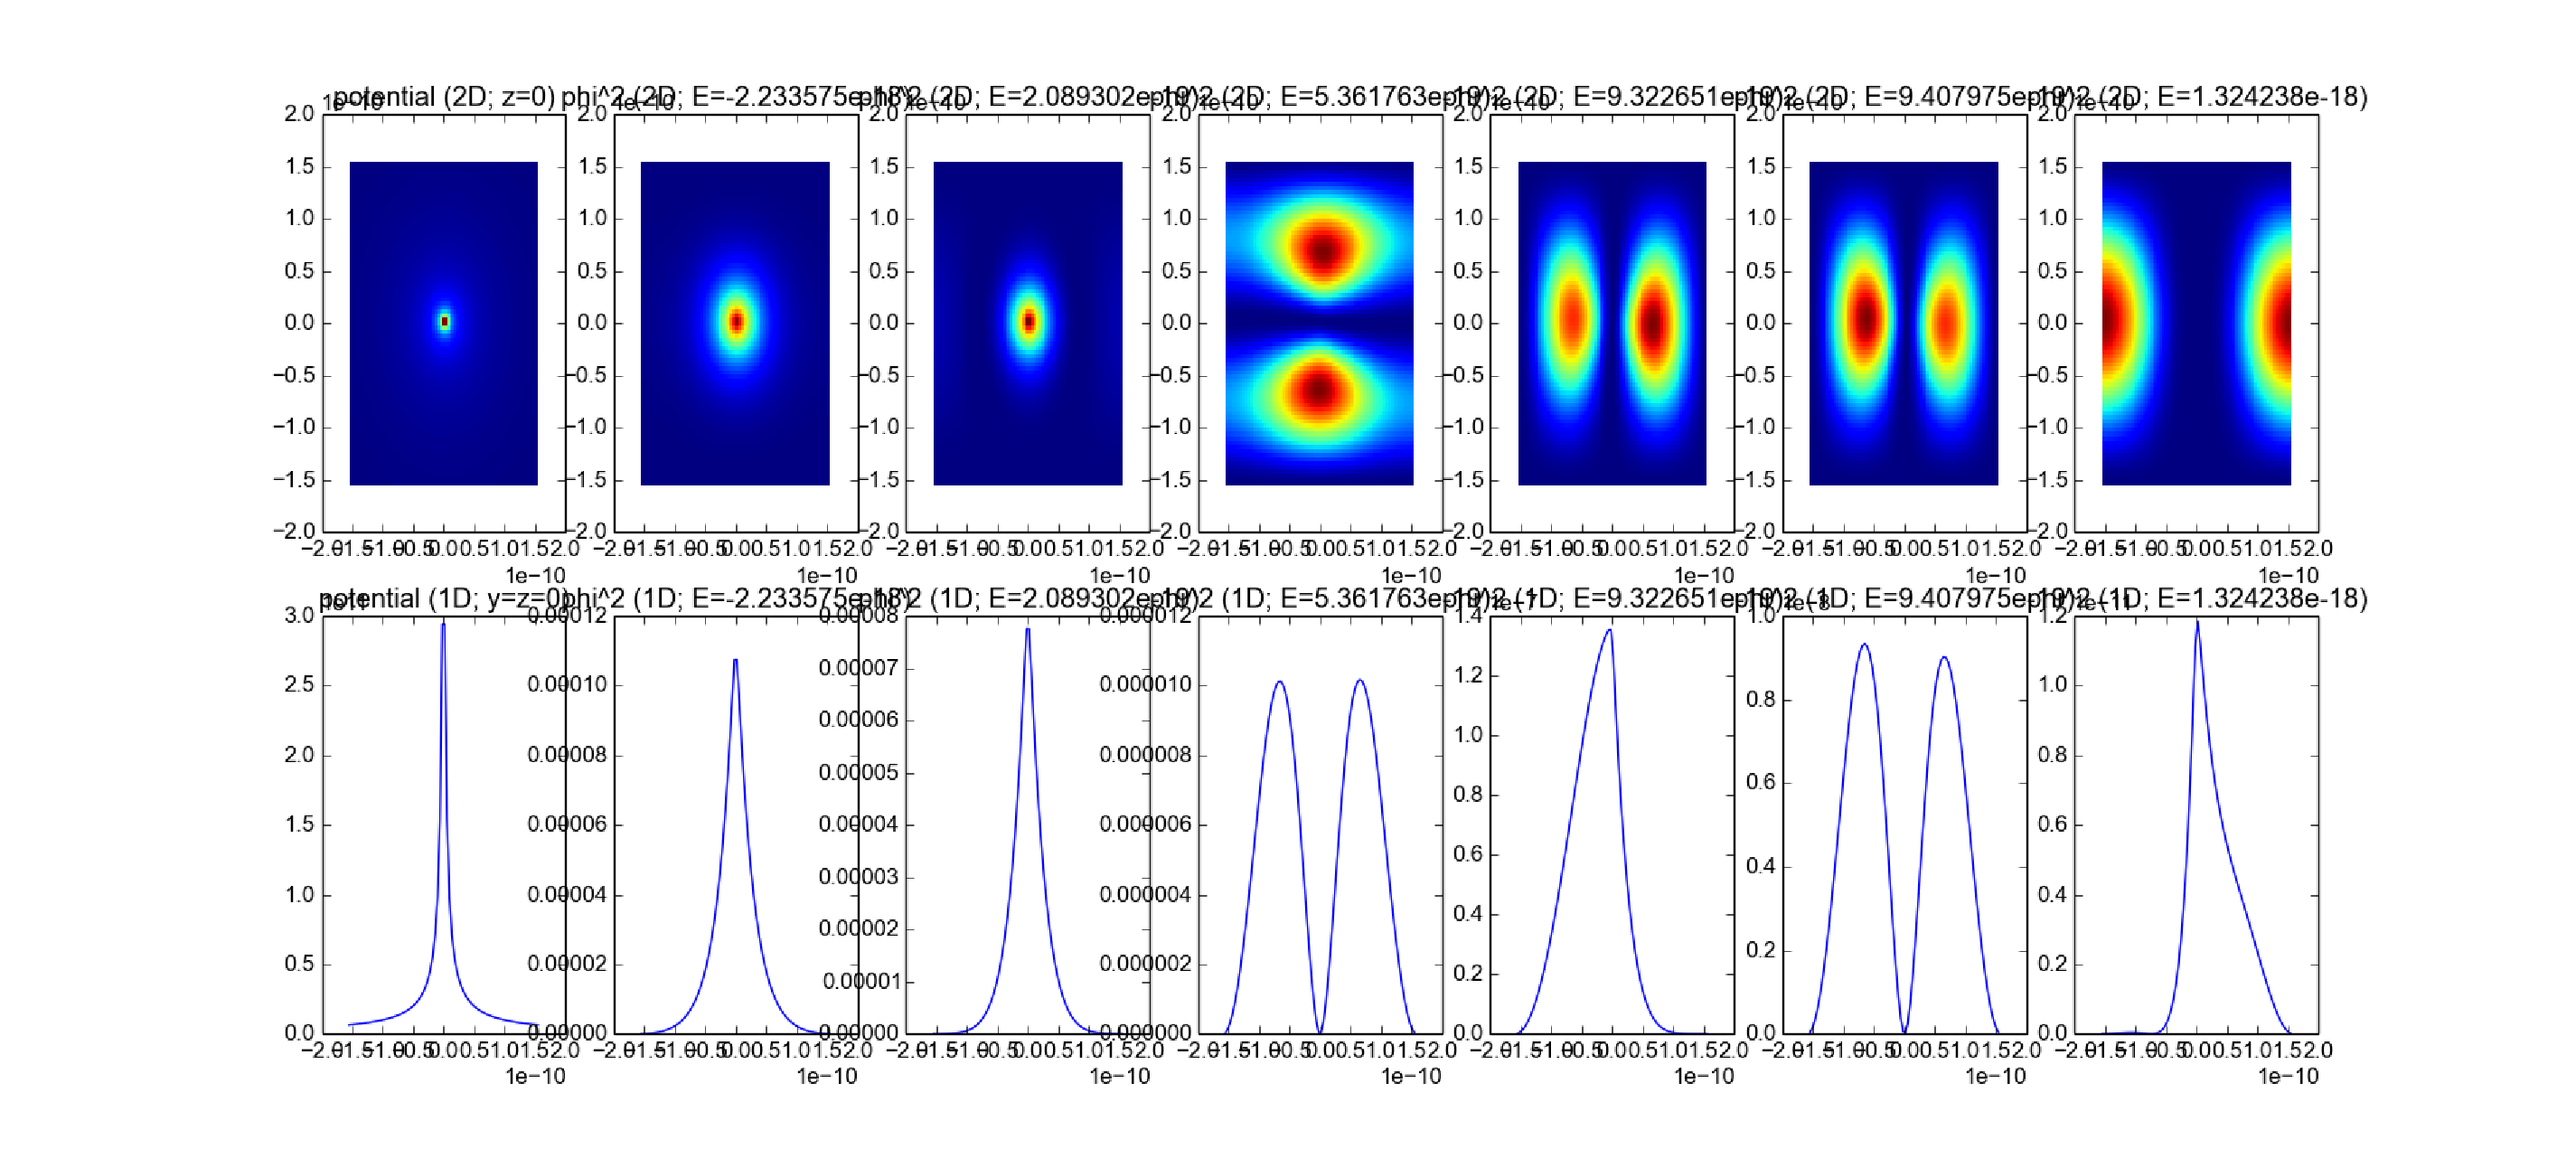
\includegraphics[width=\textwidth]{out/pdf/img/hydrogen_80.pdf}

なお,最小の固有値は,$-2.23308690\times 10^{-18}$ [J]と出ており,
これは「水素原子 基底状態 エネルギー」とかでググって出てくる値と
近いもので,いいのではないかという気がしています.

\appendix

\section{7/1時点のコード}
実質的な仕事をしているのは {\tt make\_lhs\_matrix}
という 10文ほどの関数.

\lstinputlisting[]{../hydrogen.py}


\end{document}
